\documentclass[aspectratio=169]{beamer}
\mode<presentation>{
  \usetheme{default}
  \usecolortheme{dove}
}
\defbeamertemplate*{footline}{my footline}
{
	\ifnum \insertpagenumber=1
		\leavevmode%
		
\includegraphics[width=\paperwidth]{MPIM_Titelseite_unten.pdf}%NEW
		\vskip-10pt%NEW
		\hbox{%
			\pgfsetfillopacity{0}\begin{beamercolorbox}[wd=1\paperwidth,ht=2.25ex,dp=1ex,center]{title in head/foot}%
				\usebeamerfont{title in head/foot}\pgfsetfillopacity{1}%\insertframenumber{} / \inserttotalframenumber\hspace*{2ex}
			\end{beamercolorbox}%
		}%
		\vskip0pt%
	\else
		\leavevmode%
		%
\includegraphics[width=\paperwidth]{MPIM_IMPRS_Folgeseite_unten.pdf}
		
\includegraphics[width=\paperwidth]{MPIM_Titelseite_unten.pdf}		
		\vskip-10pt
		\hbox{%
			\pgfsetfillopacity{0}\begin{beamercolorbox}[wd=1\paperwidth,ht=2.25ex,dp=1ex,center]{title in head/foot}%
				\usebeamerfont{title in head/foot}\pgfsetfillopacity{1}\insertframenumber{} / \inserttotalframenumber\hspace*{2ex}
			\end{beamercolorbox}%
		}%
		\vskip0pt%
	\fi
}

\setbeamertemplate{navigation symbols}{}%remove navigation symbols

%\usepackage[colorlinks=true, urlcolor=blue, linkcolor=blue,citecolor=blue]{hyperref}
%\usepackage[german]{babel}
\usepackage{float}
%\usepackage[numbers]{natbib}
\usepackage[authoryear]{natbib}
\definecolor{links}{HTML}{2A1B81}
\hypersetup{colorlinks,linkcolor=links,urlcolor=links}
\usepackage{appendixnumberbeamer}

%\let\oldcite=\cite                                                              
%\renewcommand{\cite}[1]{\textcolor[rgb]{.7,.7,.7}{\oldcite{#1}}}

\usepackage{graphicx}
\graphicspath{{/home/mpim/m300524/MSc_Thesis/gfx/}}

%\newcommand{\member}{m105_1994_2001}
\newcommand{\member}{m178_1985_1992} % zweitbesten
%\newcommand{\member}{m182_1988_1995} %funktioniert am besten

\renewcommand\refname{References and Notes}


\makeatletter
\setbeamertemplate{footline}[my footline]





%\title{\vspace{1cm} \\ Internal variability of the Southern Ocean carbon sink in MPI-ESM large ensemble simulations: perspective from responses of ocean biology and circulation to westerly wind changes}
\title{\vspace{5mm} \\ Internal variability of the Southern Ocean carbon sink in MPI-ESM large ensemble simulations: \\ assessment of westerly wind changes}

\subtitle{ \vspace{1cm} Aaron Spring,$^{1}$ Hongmei Li,$^{1}$ Tatiana Ilyina$^{1}$
\\ \normalsize{$^{1}$Max Planck Institute for Meteorology, Bundesstra{\ss}e 53, 20146 Hamburg, Germany}
}



\begin{document}
\begin{frame}[noframenumbering]
	\titlepage
\end{frame}

\section{Introduction}
\begin{frame}{Observations \citep{landschuetzer2015} show an anomalous decadal outgassing trend in the Southern Ocean carbon sink in the 1990s.}
	\begin{figure}[h]
	\centering
	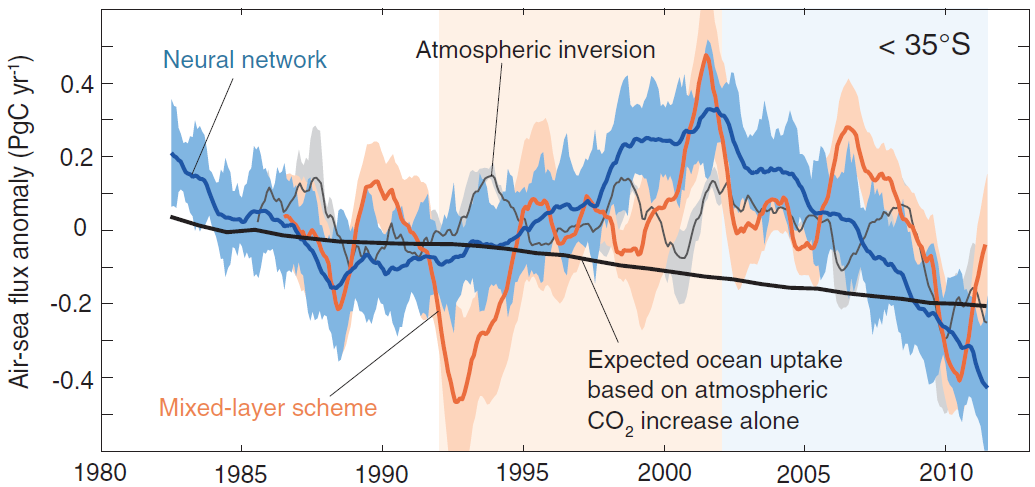
\includegraphics[scale=.3]{landschuetzer_fig1.png} % from gfx folder
	%\caption{Southern Ocean CO$_2$flux where negative values indicate ocean uptake (top) and primary production (bottom): ensemble median (left) as forced signal and ensemble standard deviation (right) as internal variability}
	\label{fig:SOCS_ensmean_ensstd}
	\end{figure}
	
\end{frame}
	
	
\section{Method}
\begin{frame}{Decadal trends of internal variability were not yet explored in coupled earth system models. We use initially perturbed 100-member historical ensemble simulations to assess the variability of the Southern Ocean carbon sink and its underlying processes.}
%I identify similar decadal trends in the MPI-ESM LE.	

	\begin{figure}
		\centering
		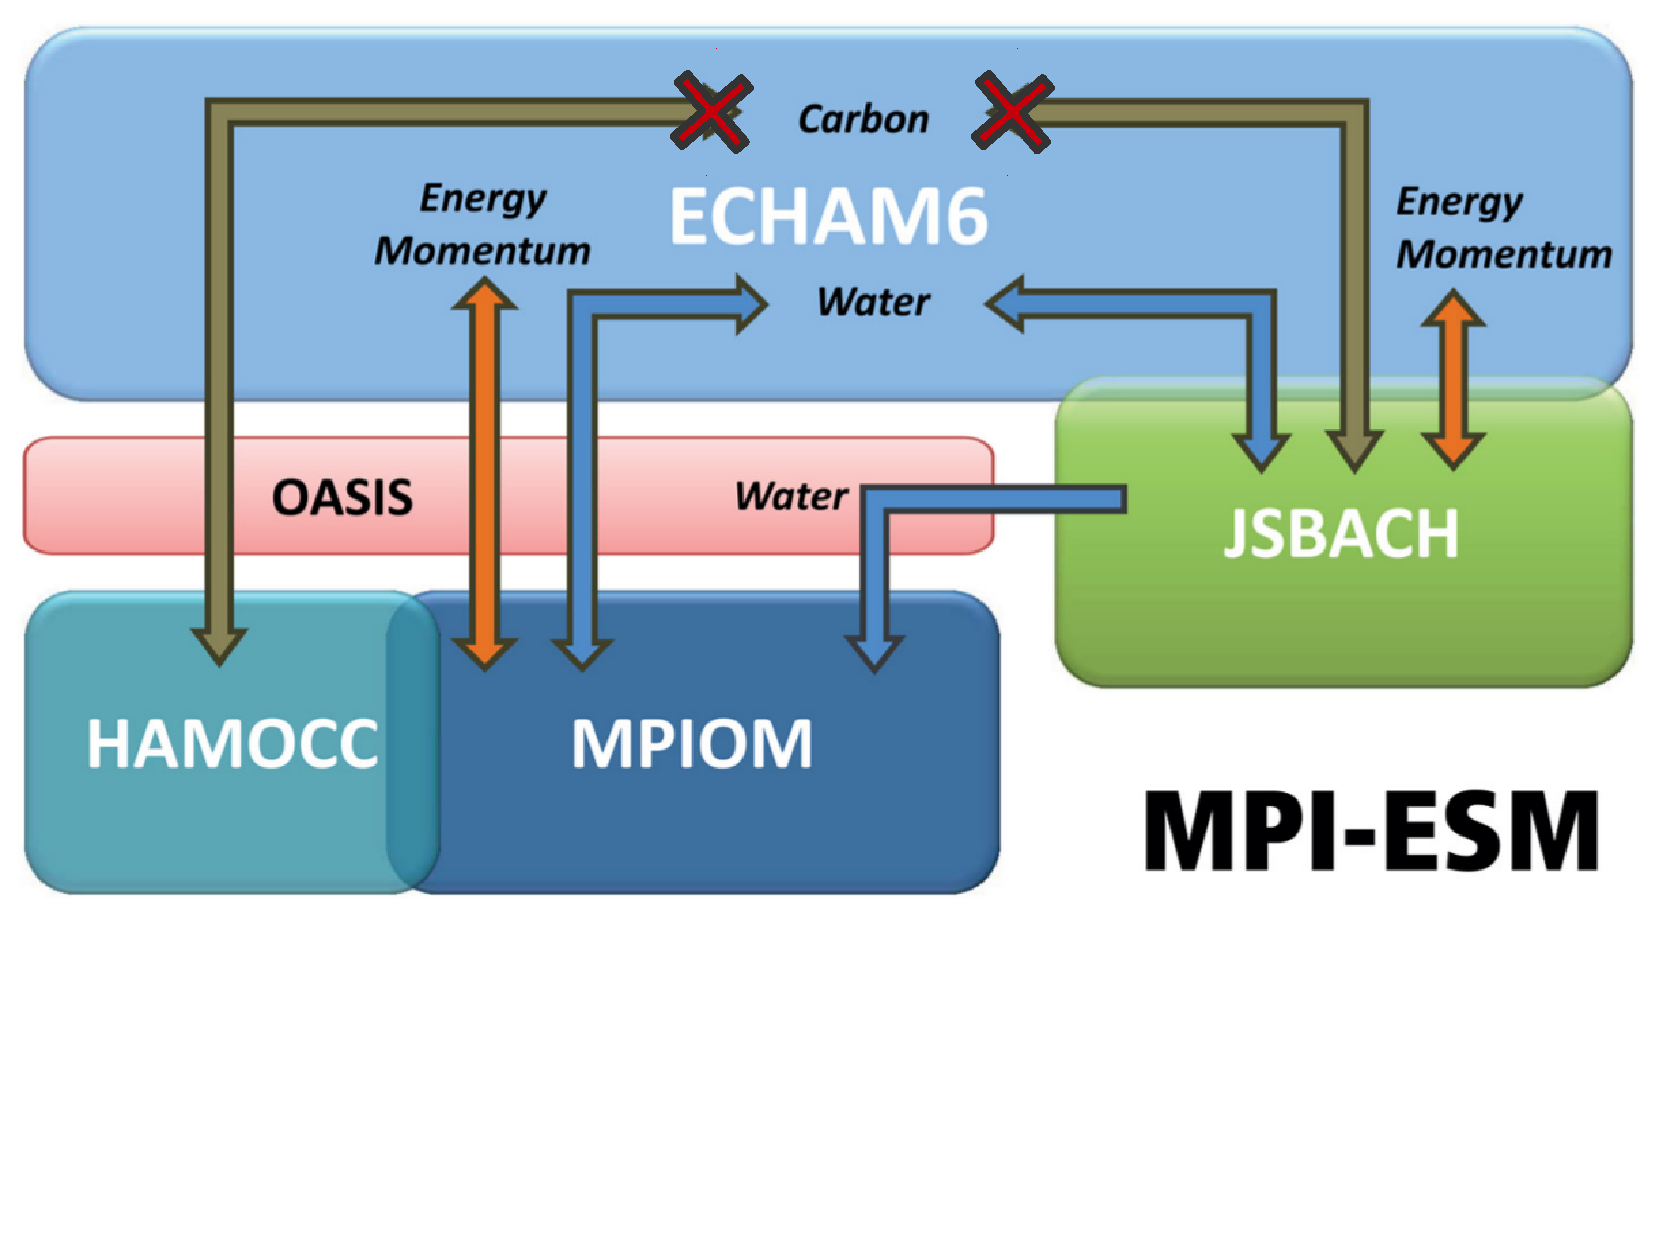
\includegraphics[scale=.28,trim=0cm 6cm 0cm 0cm,clip]{MPIESM.pdf}
		\caption{Schematic view of MPI-ESM1.1 with a diagnostic carbon cycle}
	\end{figure}
\end{frame}

\section{Scientic questions}
\begin{frame}{Scientific questions}
\Large
	\begin{enumerate}
	\item How large is the modeled decadal internal variability in the Southern Ocean carbon sink?
	\item Do we find similar trends to those observed in the 1990s and 2000s in this large ensemble?
	\item Which processes drive decadal internal variability in this large ensemble?
	\end{enumerate}
\end{frame}

\section{Results}
\begin{frame}{The modeled internal decadal variability is $\pm$0.36 PgC (2$\sigma$ ensemble standard deviations). We find positive decadal trends in the Southern Ocean carbon sink similar to observations in the 1990s. } 
	\vspace{-.2cm}
	\begin{figure}
		\centering
		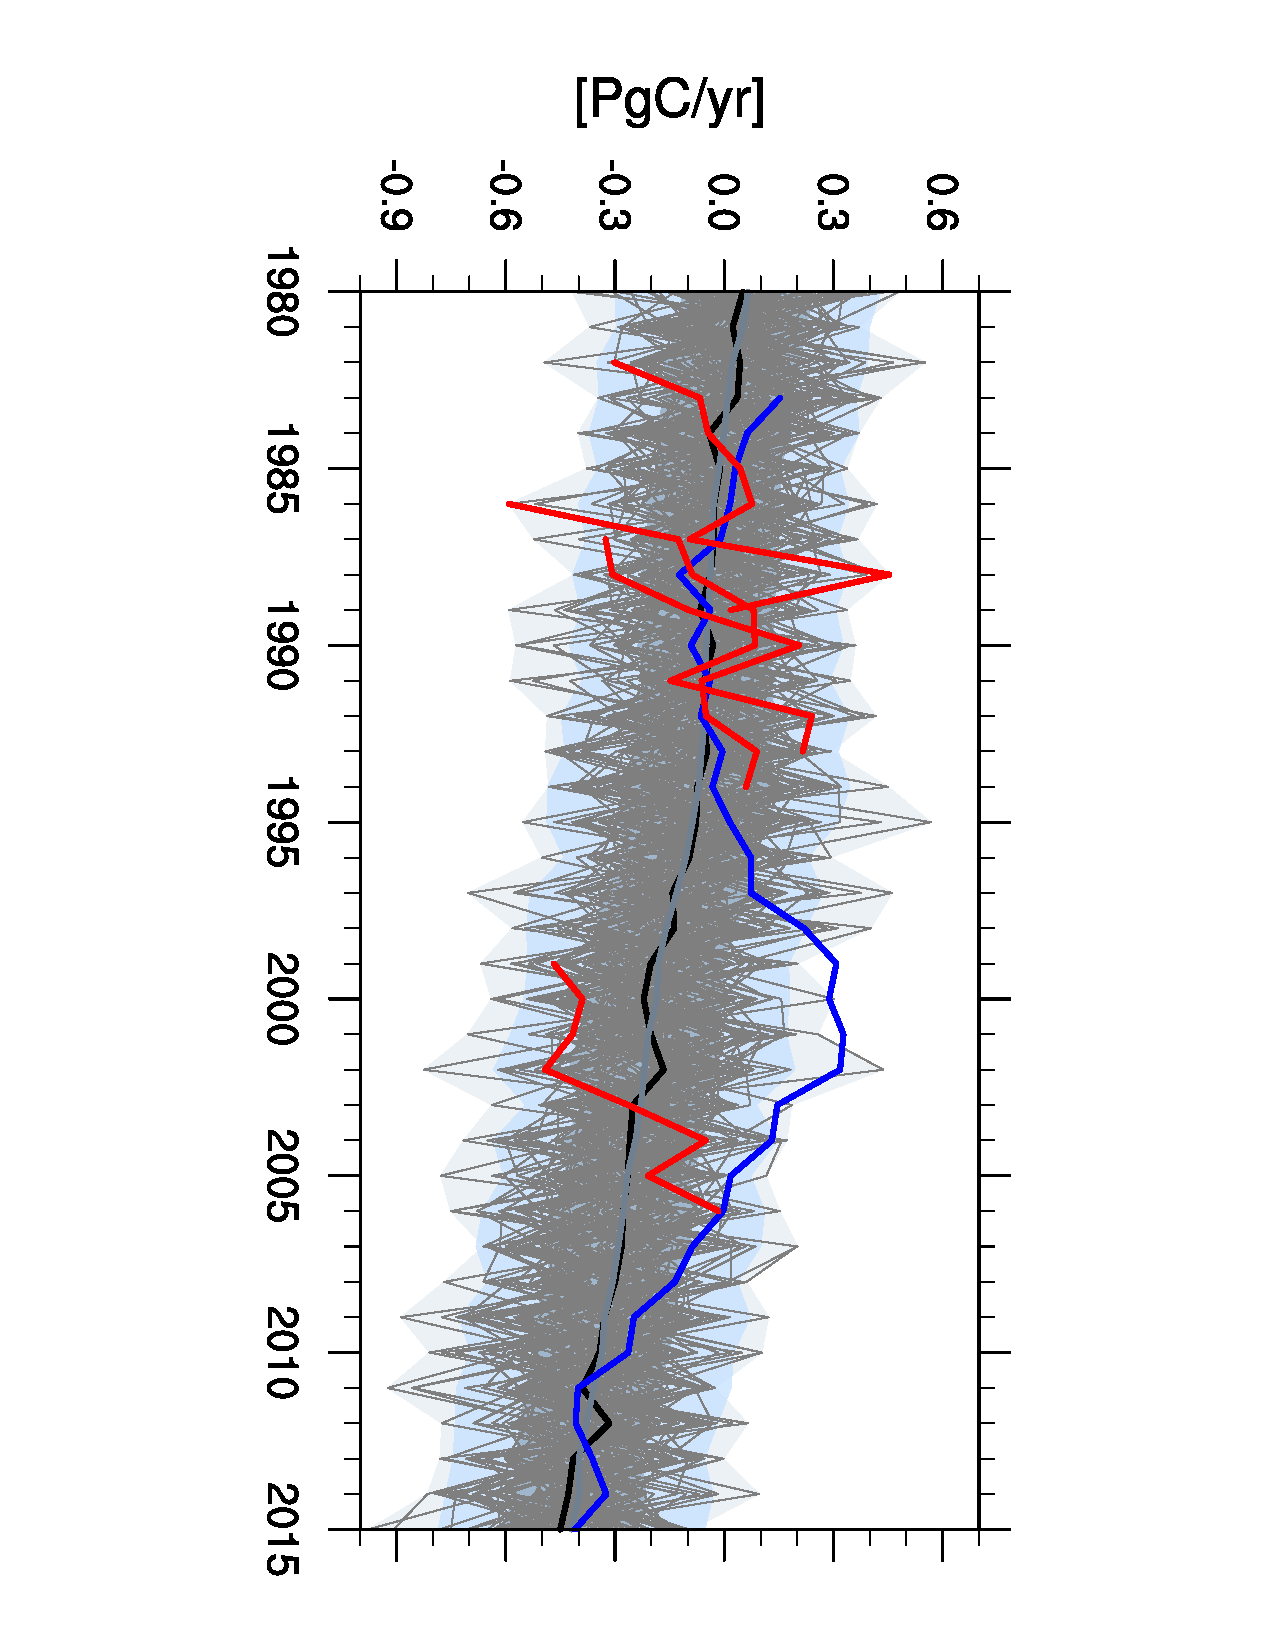
\includegraphics[scale=.28,angle=90,trim=4.5cm 0cm 4cm 0cm,clip]{co2flux_SO_timeseries_ym_mar-feb_35S_1980_2015_trend_8.pdf}
\vspace{-.2cm}		
		\caption{Evolution of the Southern Ocean carbon sink anomaly south of 35$^\circ$S. Grey lines show the 100 ensemble members, the black line the ensemble median, the gray shading is the range of the ensemble, the blue shading is the 2$\sigma$ ensemble spread, the red lines are members of decreasing sink trends, the blue line is the SOM-FFN observation-based estimate; negative values indicate anomalous uptake with respect to the 1980s}
	\end{figure}
\end{frame}	

\begin{frame}{We find westerly winds as the main driver of internal variability in the Southern Ocean carbon sink and analyze the response of biology and ocean circulation.}
	\begin{figure}
	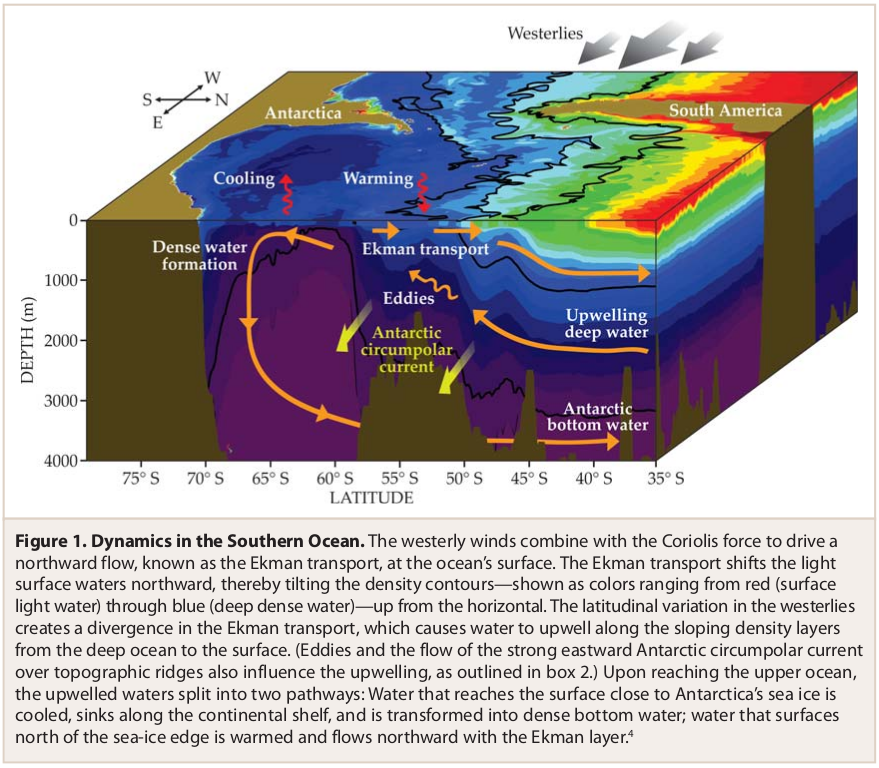
\includegraphics[scale=.4,trim=.3cm 6.8cm .5cm .5cm,clip]{Southern_Ocean_Circulation}
\vspace{-2mm}
	\caption{Dynamics of the Southern Ocean \citep{Morrison2015}}
	\end{figure}
\end{frame}
	
%not nessessarily needed	
%\begin{frame}{Internal Variability of CO$_2$flux and primary production show similar patterns, have highest values at 45-60$^\circ$S south and appear in same locations.}  
	
%	\begin{figure}
%		\centering
%		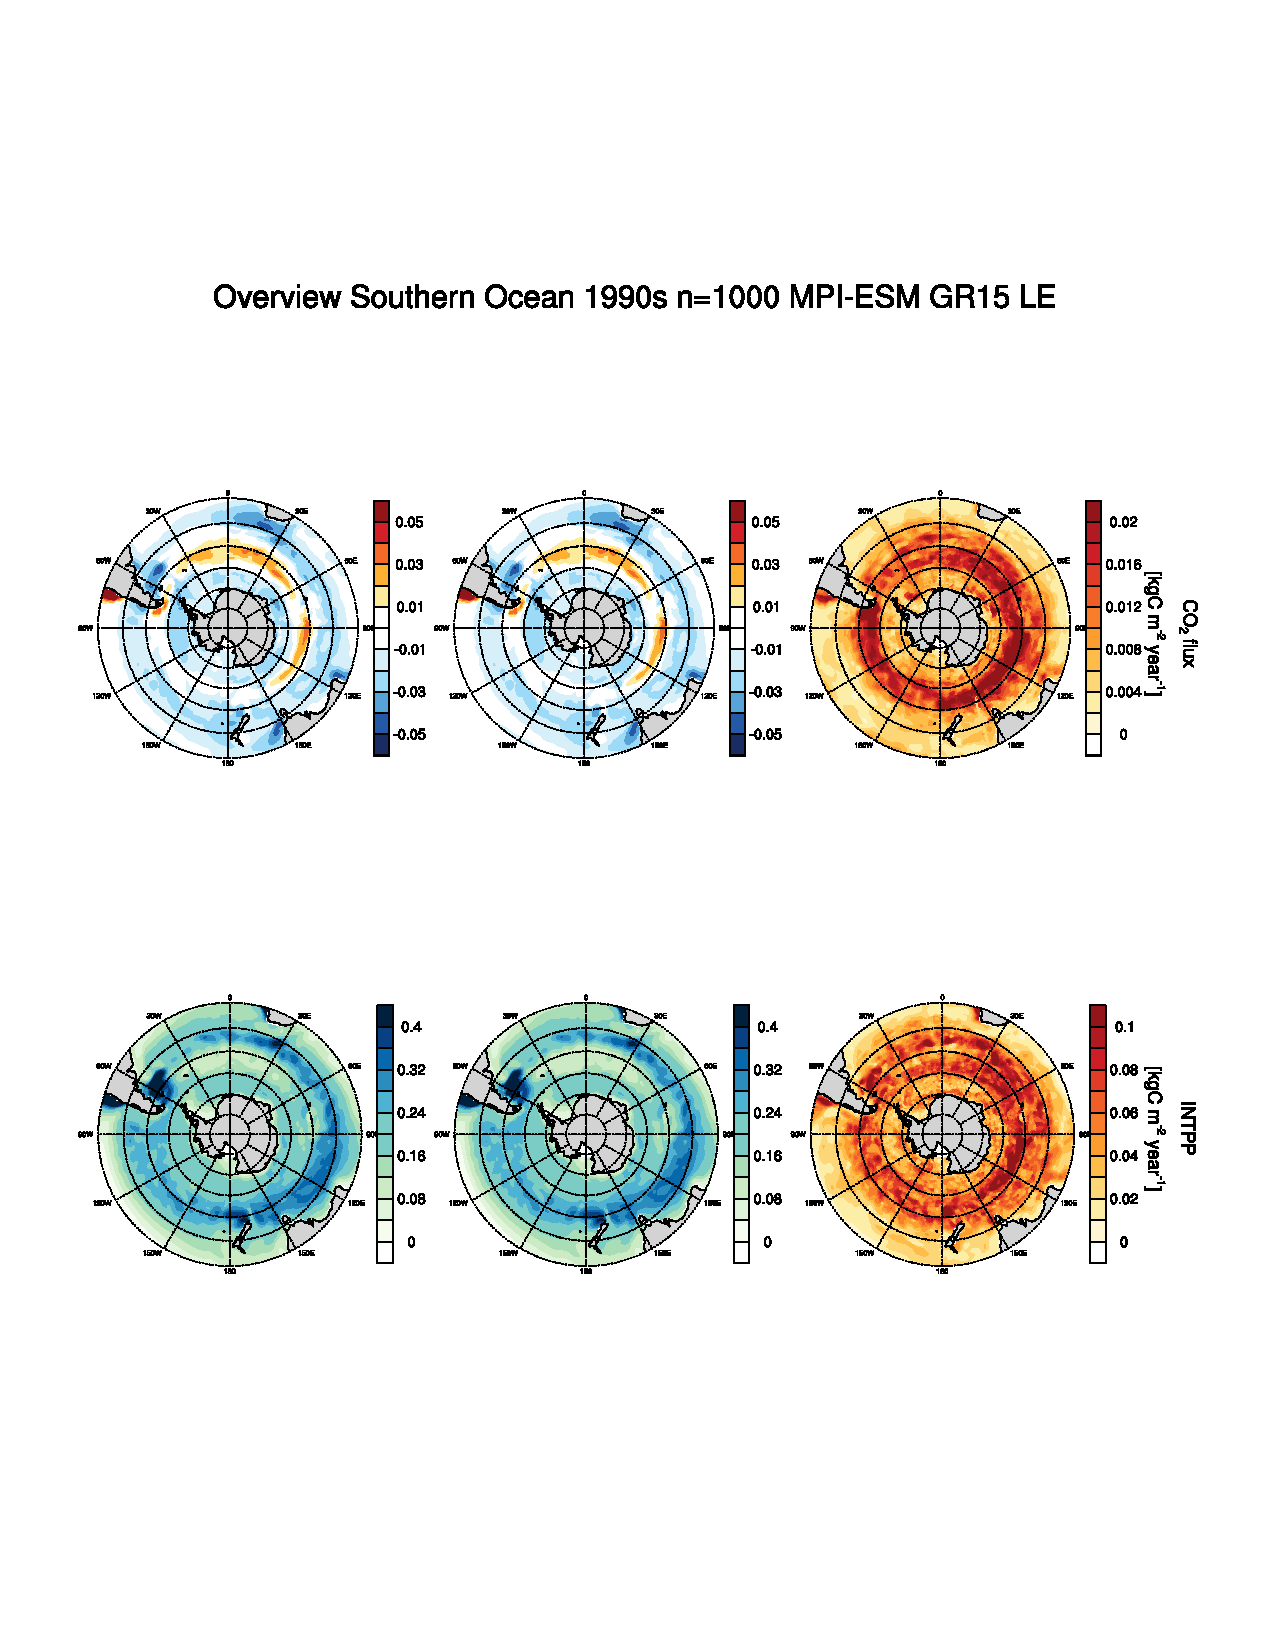
\includegraphics[scale=.45,trim=7.2cm 15cm 0cm 8cm,clip]{Overview_SO_co2flux_intpp_ens_t1990s.pdf} % from gfx folder
%		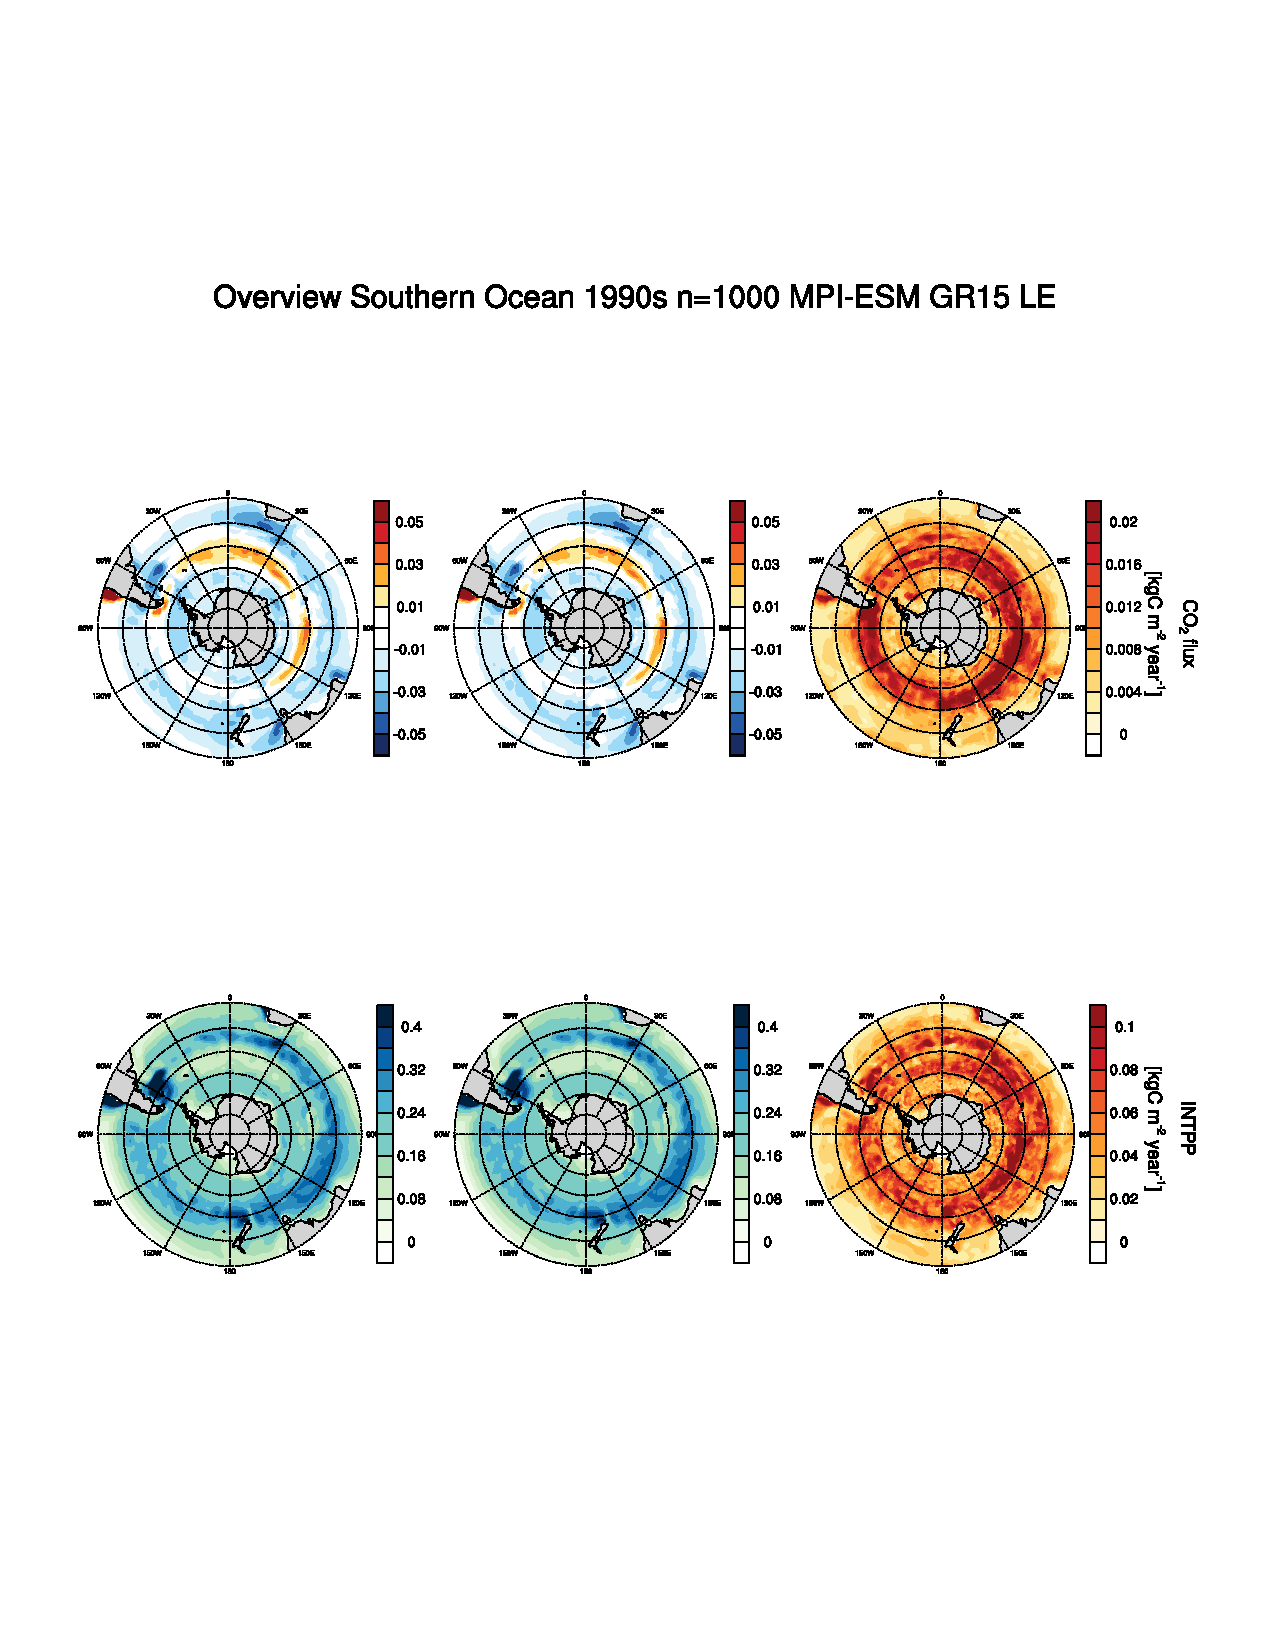
\includegraphics[scale=.45,trim=7.2cm 6.3cm 0cm 16cm,clip]{Overview_SO_co2flux_intpp_ens_t1990s.pdf} % from gfx folder
%	\caption{Southern Ocean CO$_2$flux where negative values indicate ocean uptake (1$^{st}$) and primary production (2$^{nd}$): ensemble median (left) as forced signal and ensemble standard deviation (right) as internal variability \citep{Deser2012}}
%		\label{fig:SOCS_ensmean_ensstd}
%	\end{figure}
%\end{frame}	
	
	
\subsection*{Biology}
\begin{frame}{We find correlations of significant trends in CO$_2$flux, primary production and mixed-layer depth.}
	
	\begin{figure}
		\centering
		\vspace{-2mm}
		\includegraphics[scale=.8,trim=13.25cm 18.7cm 2.5cm 6cm,clip]{\member _positive_trend_8_obgc_overview_summer.pdf} %co2flux
\includegraphics[scale=.8,trim=13.25cm 15.9cm 2.5cm 9.2cm,clip]{\member _positive_trend_8_obgc_overview_summer.pdf} %intpp

\includegraphics[scale=.8,trim=13.25cm 13.1cm 2.5cm 12.1cm,clip]{\member _positive_trend_8_obgc_overview_summer.pdf} %nutlimf
\includegraphics[scale=.8,trim=13.25cm 7.3cm 2.5cm 17.8cm,clip]{\member _positive_trend_8_obgc_overview_summer.pdf} %zmld
\caption{Southern Ocean austral summer trends over 8 years: CO$_2$flux (top left), vertically integrated primary production (top right), surface nutrient limitation (bottom left) and mixed layer depth (bottom right); hatched areas indicate where trends were below 95\% significance}
\label{fig:co2flux_intpp}
	\end{figure}
\end{frame}	

\begin{frame}{Light limitation causes the decline in primary production at 50-60$^\circ$S. Phytoplankton gets mixed deeper into the ocean.} %\citep{Sverdrup1953}.}

	\begin{figure}
		\centering
		\includegraphics[scale=.6,trim=10.5cm 13.2cm 0cm 7cm,clip]{\member _positive_trend_8_schwerpunkt_mixing_overview.pdf} 
		\includegraphics[scale=.6,trim=1.2cm 13.2cm 11cm 7cm,clip]{\member _positive_trend_8_schwerpunkt_mixing_overview.pdf}
\caption{Trends in [m/8yrs] of average depth of vertical diffusivity due to wind (left) and for phytoplankton average depth (right); hatched areas indicate where trends were below 95\% significance}
\label{fig:wind_mixing}
	\end{figure}
	
\end{frame}


\begin{frame}{Deeper winter mixing delays primary production blooms in austral spring and lowers primary production all over the summer.}
	\begin{figure}[h]
		\centering
		\includegraphics[page=2,scale=.3,trim=0cm 6cm 0cm 5cm,clip]{\member _positive_trend_8_seasonality_intpp_zmld.pdf} % from gfx folder
		\caption{Seasonality of vertically integrated primary production (black) and mixed layer depth (red) at 50-60$^\circ$S over 8 years; thicker lines are later years}
		\label{fig:zmld_intpp_seasonality}
	\end{figure}
	
\end{frame}

\begin{frame}{Previous studies show increasing primary production for increasing winds. Increased upwelling brings more nutrients, but this has no effect on biology in HAMOCC.}
\begin{figure}
\centering
\vspace{-.5cm}
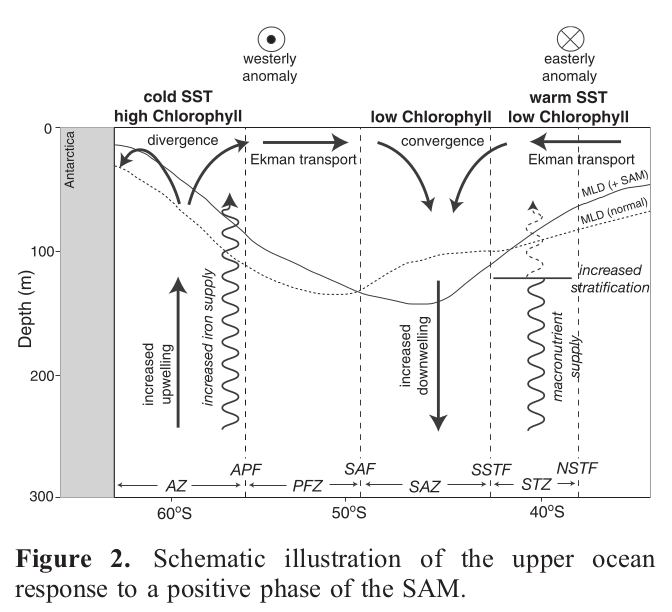
\includegraphics[scale=.3,trim=0cm 2.3cm 0cm .7cm,clip]{Southern_Ocean_SAM_zmld_response_Lovenduski2005}
\includegraphics[scale=1.2,trim=5.8cm 13.1cm 12cm 12.1cm,clip]{\member _positive_trend_8_obgc_overview_summer.pdf} %nutlimf
\includegraphics[scale=1.2,trim=13.25cm 13.1cm 4.3cm 12.1cm,clip]{\member _positive_trend_8_obgc_overview_summer.pdf} %nutlimf
\caption{(left) Schematic view of the upper ocean
response to a positive SAM phase \citep{Lovenduski2005}; (right) surface nutrient limitation function summer mean and trend} 
\end{figure}
\vspace{-3mm}
related papers: \citep{Lovenduski2008} \citep{wang2012} \citep{Hauck2013} 
\end{frame}

\subsection{Circulation}
\begin{frame}{Upper-ocean overturning circulation is strengthened by intensified westerly winds. Increased upwelling south of 50$^\circ$S brings more carbon-rich waters to the surface.}
\begin{figure}
\vspace{-5mm}
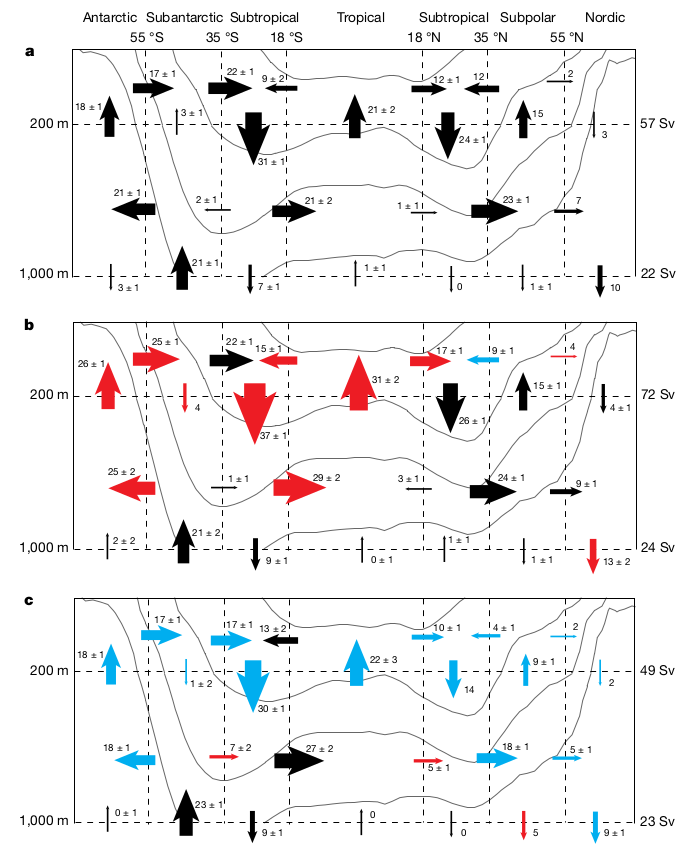
\includegraphics[scale=.33,trim=0.5cm 7.2cm 0cm .2cm,clip]{DeVries_2017_Fig1_Upper_Ocean_Overturning_Circulation}
\includegraphics[scale=.8,trim=13.25cm 18.7cm 2.5cm 6cm,clip]{\member _positive_trend_8_obgc_overview_winter.pdf} %co2flux
\includegraphics[scale=.8,trim=13.25cm 15.9cm 2.5cm 9.2cm,clip]{\member _positive_trend_8_obgc_overview_winter.pdf} %wmo
\vspace{-3mm}
\caption{(left) Upper-ocean overturning circulation (a: normal; b: stronger winds) \citep{DeVries2017}; (right) trends in winter in CO$_2$flux and advective upward transport}
\end{figure}
\end{frame}


\section{Conclusion}
\begin{frame}{The strength of westerly winds dominates the internal variability of the Southern Ocean carbon sink. The explained mechanisms apply vice versa for decreasing winds .}
\vspace{-.7cm}
	\begin{figure}
		\includegraphics[scale=.28,page=2,angle=90,trim=1.3cm 2.3cm 2.3cm 3cm,clip]{Scatter_trends_ensanom_co2flux_vs_SAM_n1800_1980_1997}
		
		\vspace{-2mm}
		\caption{Southern Annular Mode (SAM) as indicator of wind strength vs. CO$_2$flux south of 35$^\circ$S; one data point represents 8-year trends of single realization minus ensemble mean in 8-year periods between 1980 and 2005}
	\end{figure}
\end{frame}

\begin{frame}{Questions now}
\begin{itemize}
\Large
\item Are the research questions answered?
\item Can I quantify internal variability as $\pm$ 2$\sigma$ ensemble standard deviations? 
\item Can I call biology a driver of the internal variability of the Carbon Sink or is it rather the response of biology to the westerly winds which are the driver?
\item Upwelling nutrients don't change primary production: iron-hypothesis for Southern Ocean doesn't apply in HAMOCC?
\item Is this scatter plot useful to show the link between winds and CO$_2$flux in general?
\end{itemize}
\end{frame}
	
\appendix

\begin{frame}[allowframebreaks]{References}
\baselineskip12pt
\bibliography{../Paper/SouthernOceanCarbonSink_new}

\bibliographystyle{abbrvnat}%unsrtnat}%abbrvnat}%plainnat}

\end{frame}	
	
	
	
\end{document}